\section{Einleitung}

\section{Team}

\begin{frame}
    \frametitle{\insertsection}
    \vfill
    \begin{columns}
        \begin{column}[c]{0.2\textwidth}
            
\includegraphics[height=3em]{fig/logo_ess}  
        \end{column}
        \begin{column}[c]{0.7\textwidth}
            \textbf{Fachgebiet Elektrische Systeme \& Sensorik}\\
            LG3A, 1. Stock, Siemens-Halske-Ring 14, Cottbus
        \end{column}
    \end{columns}
    
    \vfill

    \begin{columns}[onlytextwidth]
        \begin{column}{0.5\textwidth}
            \textbf{Vorlesung:} Prof. Dr.-Ing. Markus Gardill
            \begin{itemize}
                \item markus.gardill@b-tu.de
                \item Tel.: 0355 69-3410
            \end{itemize}
            \begin{center}
                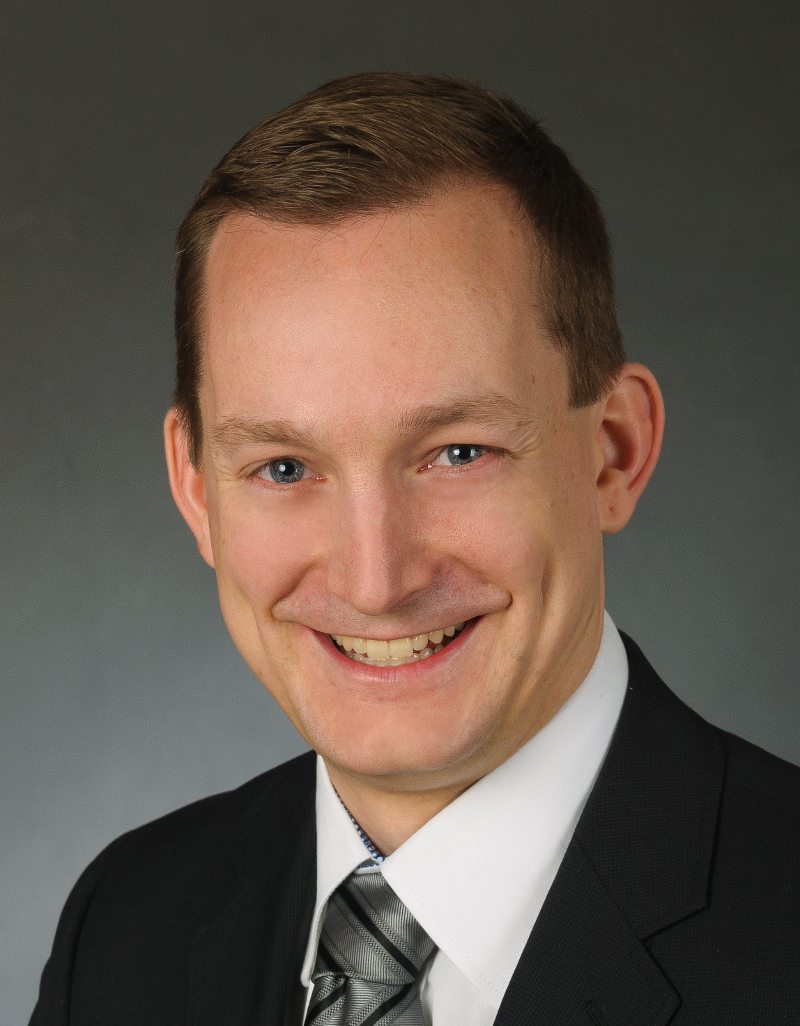
\includegraphics[height=3cm]{fig/photo_gardill}
            \end{center}
        \end{column}
        \begin{column}{0.5\textwidth}
            \textbf{Übung:} Dipl.-Ing. Marcus Heide
            \begin{itemize}
                \item marcus.heide@b-tu.de
                \item Tel.: 0355 69-3425
            \end{itemize}
            \begin{center}
                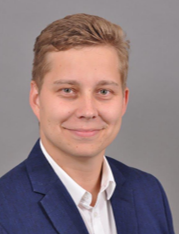
\includegraphics[height=3cm]{fig/photo_heide}
            \end{center}
        \end{column}
    \end{columns}

\end{frame}